% Nancy User’s Guide

\documentclass[a4paper,english]{scrartcl}
\usepackage{babel,a4,newlfont,fancyvrb,copyrght,graphicx}
\usepackage[utf8]{inputenc}

% New commands
\renewcommand{\copyrightyear}{2002--2016}

\begin{document}

\title{Nancy, the lazy weaver\\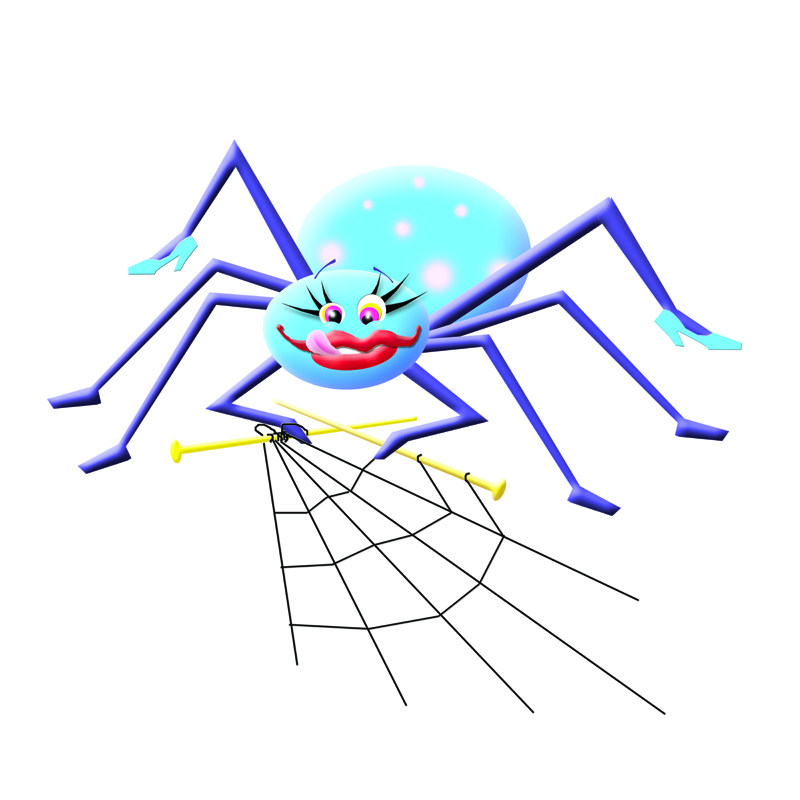
\includegraphics[scale=0.45]{logo/nancy.png}
\\User’s guide}
\date{21st February 2016}
\author{Reuben Thomas}
\maketitle

\section{Introduction}

Nancy is a simple macro processor that weaves files together out of other files. File content can be generated programmatically.

\section{Invocation}

Nancy takes two arguments:

\begin{verbatim}
nancy [OPTION...] PATH TEMPLATE
\end{verbatim}

\noindent where \verb|PATH| is the path of the file or directory to weave, and \verb|TEMPLATE| is name of the template file.

The following command-line \verb|OPTION|s may be given:

\begin{description}
\SaveVerb{root}|--root DIRECTORY|
\item[\UseVerb{root}]Set the source root directory (the default is the current directory).
\SaveVerb{listfiles}|--list-files|
\item[\UseVerb{listfiles}]List on standard error the files used to make each page.
\SaveVerb{version}|--version|
\item[\UseVerb{version}]Show the version number of Nancy.
\SaveVerb{help}|--help|
\item[\UseVerb{help}]Show help on how to run Nancy.
\end{description}

The options may be abbreviated to any unambiguous prefix.

\section{Operation}
\label{operation}

Nancy weaves a path given a template as follows:

\begin{enumerate}
\item Set the initial text to \verb|$include{TEMPLATE}|.
\item Repeatedly scan the text for a command and replace it by its output, until no more commands are found.
\item Output the resultant text.
\end{enumerate}

A command takes the form \verb|$COMMAND| or \verb|$COMMAND{ARGUMENT, ...}|.

Nancy recognises these commands:

\begin{description}
\SaveVerb{include}|$include{FILE, ARGUMENT, ...}|
\item[\UseVerb{include}]Look up the given file. If it is executable, run it as a command with the given arguments and replace the command with the output of the command. Otherwise, replace the command with the contents of the given file.
\SaveVerb{path}|$path|
\item[\UseVerb{path}]Replace the command with the \verb|PATH| argument.
\SaveVerb{path}|$root|
\item[\UseVerb{path}]Replace the command with the root directory.
\SaveVerb{path}|$template|
\item[\UseVerb{path}]Replace the command with the \verb|TEMPLATE| argument.
\end{description}

The last three commands are mostly useful as arguments to \verb|$include|.

Only one guarantee is made about the order in which commands are processed: if one command is nested inside another, the inner command will be processed first. (The order only matters for \verb|$include| commands that run executables; if you nest them, you have to deal with this potential pitfall.)

To find the file \verb|FILE| specified by a \verb|$include| command, Nancy proceeds thus:

\begin{enumerate}
\item See whether \verb|ROOT/PATH/FILE| is a file (or a symbolic link to a file). If so, return the file path.
\item If not, remove the last directory from \verb|PATH| and try again, until \verb|PATH| is empty.
\item Finally, try looking for \verb|FILE|.
\item If no file is found, Nancy stops with an error message.
\end{enumerate}

For example, if the root directory is \verb|/dir|, \verb|PATH| is \verb|foo/bar/baz|, and Nancy is trying to find \verb|file.html|, it will try the following , in order:

\begin{enumerate}
\item \verb|/dir/foo/bar/baz/file.html|
\item \verb|/dir/foo/bar/file.html|
\item \verb|/dir/foo/file.html|
\item \verb|/dir/file.html|
\end{enumerate}

\section{Example: generating a web site}
% FIXME: add example use of an executable fragment (date)
% FIXME: the examples are unclear; really ought to be actual web pages with some sort of structure diagrams automatically generated

Suppose a web site has the following page design, from top to bottom: logo, navigation menu, breadcrumb trail, page body.

Most of the elements are the same on each page, but the breadcrumb trail has to show the canonical path to each page, and the logo is bigger on the home page, which is the default \verb|index.html|.

Suppose further that the web site has the following structure, where each line corresponds to a page:

\begin{itemize}
\item Home page
\item People
  \begin{itemize}
  \item Jo Bloggs
  \item Hilary Pilary
  \item \dots
  \end{itemize}
\item Places
  \begin{itemize}
  \item Vladivostok
  \item Timbuktu
  \item \dots
  \end{itemize}
\end{itemize}

The basic page template looks something like this:

\begin{verbatim}
<html>
  <link href="style.css" rel="stylesheet" type="text/css">
  <title>$include{title}</title>
  <body>
    <div class="logo">$include{logo.html}</div>
    <div class="menu">$include{menu.html}</div>
    <div class="breadcrumb">$include{breadcrumb.html}</div>
    <div class="main">$include{main.html}</div>
  </body>
</html>
\end{verbatim}

Making the menu an included file is not strictly necessary, but makes the template easier to read. The pages will be laid out as follows:

\begin{itemize}
\item \verb|/|
  \begin{itemize}
  \item \verb|index.html|
  \item \verb|people/|
    \begin{itemize}
    \item \verb|index.html|
    \item \verb|jo_bloggs.html|
    \item \verb|hilary_pilary.html|
    \end{itemize}
  \item \verb|places/|
    \begin{itemize}
    \item \verb|index.html|
    \item \verb|vladivostok.html|
    \item \verb|timbuktu.html|
    \end{itemize}
  \end{itemize}
\end{itemize}

The corresponding source files will be laid out as follows. This may look a little confusing at first, but note the similarity to the HTML pages, and hold on for the explanation!

\begin{itemize}
\item \verb|source/|
  \begin{itemize}
  \item \verb|template.html| (the template shown above)
  \item \verb|menu.html|
  \item \verb|logo.html|
  \item \verb|breadcrumb.html|
  \item \verb|index.html/|
    \begin{itemize}
    \item \verb|main.html|
    \item \verb|logo.html|
    \end{itemize}
  \item \verb|people/|
    \begin{itemize}
    \item \verb|breadcrumb.html|
    \item \verb|index.html/|
      \begin{itemize}
      \item \verb|main.html|
      \end{itemize}
    \item \verb|jo_bloggs.html/|
      \begin{itemize}
      \item \verb|main.html|
      \end{itemize}
    \item \verb|hilary_pilary.html/|
      \begin{itemize}
      \item \verb|main.html|
      \end{itemize}
    \end{itemize}
  \item \verb|places/|
    \begin{itemize}
    \item \verb|breadcrumb.html|
    \item \verb|index.html/|
      \begin{itemize}
      \item \verb|main.html|
      \end{itemize}
    \item \verb|vladivostok.html/|
      \begin{itemize}
      \item \verb|main.html|
      \end{itemize}
    \item \verb|timbuktu.html/|
      \begin{itemize}
      \item \verb|main.html|
      \end{itemize}
    \end{itemize}
  \end{itemize}
\end{itemize}

Note that there is only one menu fragment (the main menu is the same for every page), while each section has its own breadcrumb trail (\verb|breadcrumb.html|), and each page has its own content (\verb|main.html|).

Now consider how Nancy builds the page whose URL is \verb|vladivostok.html|. According to the rules given in section~\ref{operation}, Nancy will look first for files in \verb|source/places/vladivostok.html|, then in \verb|source/places|, and finally in \verb|source|. Hence, the actual list of files used to assemble the page is:

\begin{itemize}
\item \verb|source/template.html|
\item \verb|source/logo.html|
\item \verb|source/menu.html|
\item \verb|source/places/breadcrumb.html|
\item \verb|source/places/vladivostok.html/main.html|
\end{itemize}

For the site’s index page, the file \verb|index.html/logo.html| will be used for the logo fragment, which can refer to the larger graphic desired.

% FIXME: explain how to build the web site statically, or serve it dynamically.

This scheme, though simple, is surprisingly flexible; this simple example has covered all the standard techniques for Nancy’s use.

\end{document}
